\documentclass[a4paper, 12pt]{article}
\usepackage{graphicx}
\usepackage[utf8]{inputenc}

% Default fixed font does not support bold face
\DeclareFixedFont{\ttb}{T1}{txtt}{bx}{n}{12} % for bold
\DeclareFixedFont{\ttm}{T1}{txtt}{m}{n}{12}  % for normal

% Custom colors
\usepackage{color}
\definecolor{deepblue}{rgb}{0,0,0.5}
\definecolor{deepred}{rgb}{0.6,0,0}
\definecolor{deepgreen}{rgb}{0,0.5,0}

\usepackage{listings}

% Python style for highlighting
\newcommand\pythonstyle{\lstset{
language=Python,
basicstyle=\ttm,
morekeywords={self},              % Add keywords here
keywordstyle=\ttb\color{deepblue},
emph={MyClass,__init__},          % Custom highlighting
emphstyle=\ttb\color{deepred},    % Custom highlighting style
stringstyle=\color{deepgreen},
frame=tb,                         % Any extra options here
showstringspaces=false
}}


% Python environment
\lstnewenvironment{python}[1][]
{
\pythonstyle
\lstset{#1}
}
{}

% Python for external files
\newcommand\pythonexternal[2][]{{
\pythonstyle
\lstinputlisting[#1]{#2}}}

% Python for inline
\newcommand\pythoninline[1]{{\pythonstyle\lstinline!#1!}}

\title{Przetwarzanie strumieni danych i data science, \\ Zajęcia Zintegrowane 1}
\author{Krzysztof Rudnicki, 307585}
\begin{document} 
\maketitle 
\section{Przygotowanie maszyny wirtualnej}
    \paragraph{Przekopiowałem i uruchomiłem maszynę wirtualną z pliku .ova}
    \paragraph{Uruchomiłem serwis kafka korzystając z systemctl}
    \paragraph{Zweryfikowałem, że kafka działa (zarówno systemctl) jak i Hello World \\ \\ }
    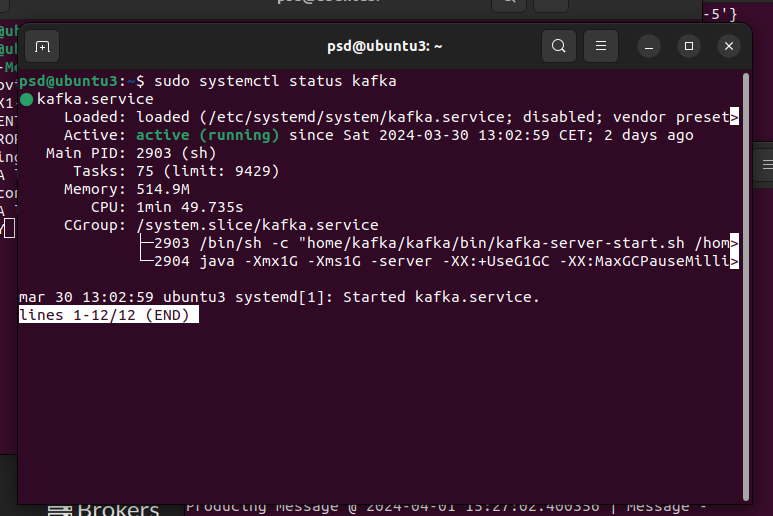
\includegraphics[width=\textwidth]{screen1.png} 
    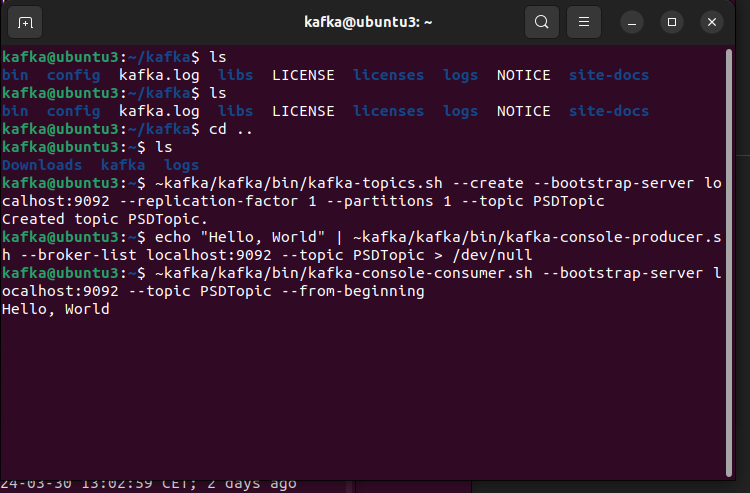
\includegraphics[width=\textwidth]{screen3.png}
    \paragraph{Uruchomiłem kafdrop \\ \\}
    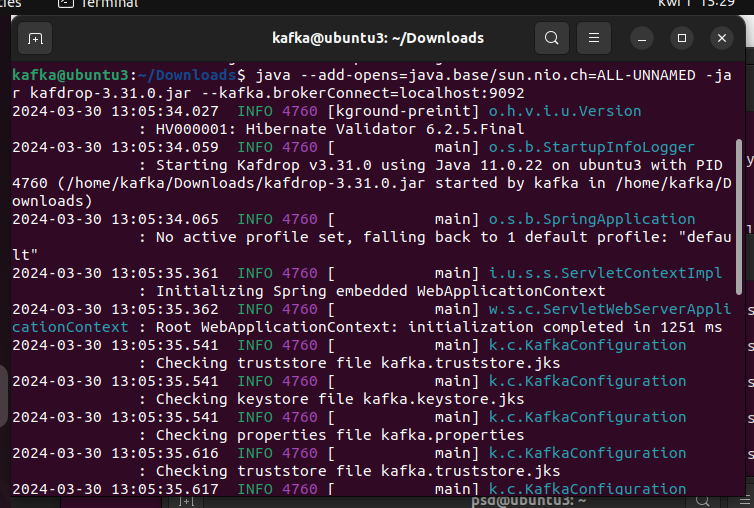
\includegraphics[width=\textwidth]{screen2.png}
    \paragraph{Przepisałem i uruchomiłem przykładowe skrypty python producenta i konsumenta \\ \\}
    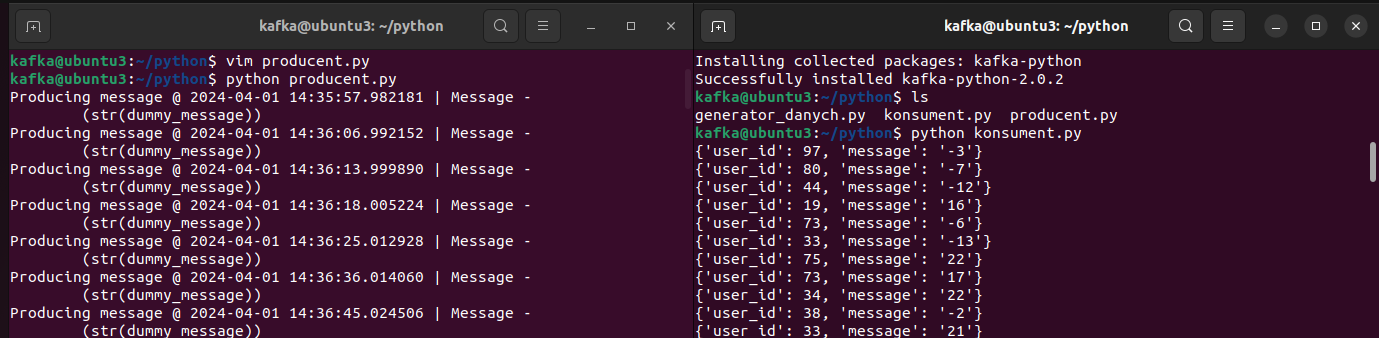
\includegraphics[width=\textwidth]{screen4.png}

\section{Przerobienie skryptu Python} 
Postanowiłem przerobić pythonowy skrypt na taki który imituje sensor temperatury  \\
Chciałem stworzyć skrypt który z jednej strony jest prosty do napisania, a z drugiej imituje faktyczną praktyczną funkcjonalność którą można by użyć na przykład przy urządzeniach internetu rzeczy \\ 
Generator danych:
\pythonexternal{simulate_temperature_sensor.py}
Producent:
\pythonexternal{producent.py}
Konsument:
\pythonexternal{konsument.py}
Przykładowe działanie: \\
\begin{center}
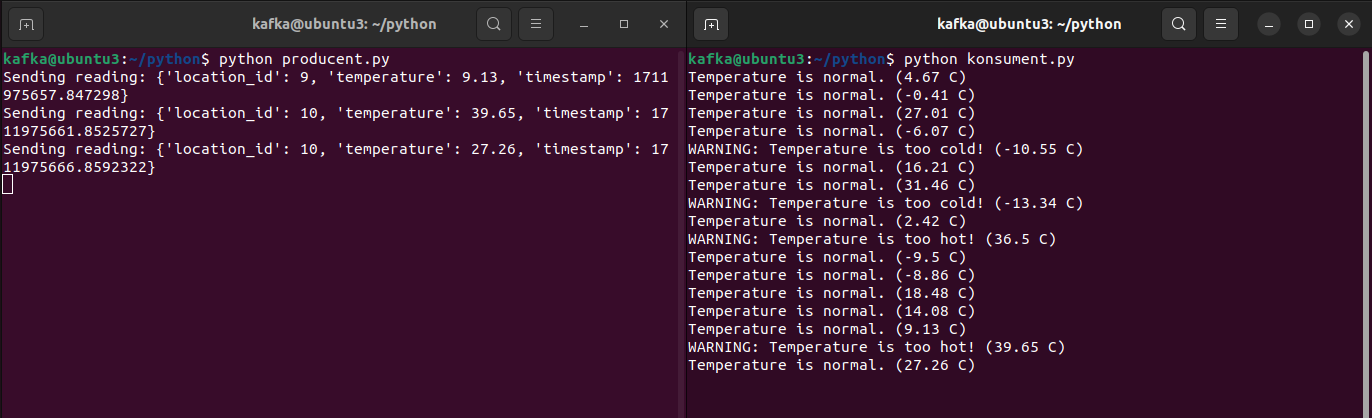
\includegraphics[width=0.8\paperwidth]{screen5.png}
\end{center}

\end{document}